\subsection{Nodal Smoothing}
For a node, $N_i$, the representation deficit is defined only by
comparing it to the node when located at another point in space. Here
the comparison is bound by limiting the range of comparison within the
edge-hull topologically adjacent to $N_i$. Formally, let $N_i$ be a node
in $D$ that is shared topologically by $n$ triangles, where $n$ is the
face-valence of $N_i$. The optimization for finding the optimal position
for $N_i$ is defined as:

\begin{eqnarray*}
\begin{array}{rcl}
\underset{N_O}{\text{minimize}} \ O(N) & = &
-\sum{_{j=1}^{n_t-1}A\left(T_j\right)} \\
\text{subject to} \ N_{T_1} & > & 0 \\
N_{T_2} & > & 0 \\ 
N_{T_3} & > & 0 \\
& \vdots & \\
N_{T_{n-1}} & > & 0 \\ 
N_{T_n} & > & 0
\end{array}
\end{eqnarray*}

\begin{figure}[h!]
  \center{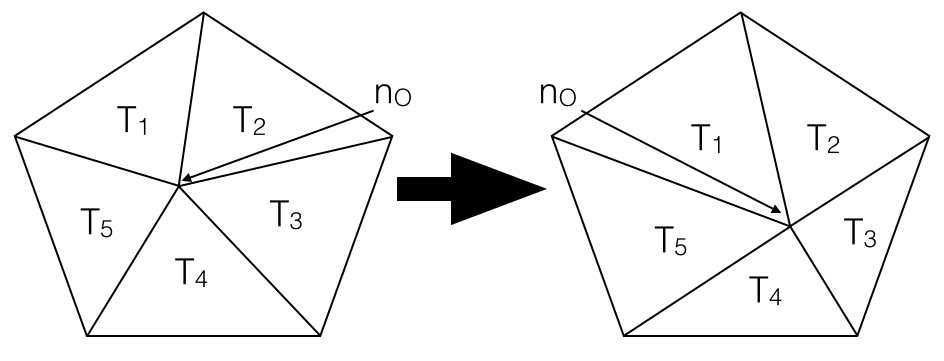
\includegraphics[height=1.4in]
    {Figures/NodalSmoothing.jpg}}
  \caption{Nodal Smoothing}
\end{figure}

[NEED TO DISCUSS HESSIAN/METRIC BASED MESH ADAPTION IN THE NODAL
SMOOTHING SECTION OF THE PAPER. THERE IS NO GLOBAL, STATIC FUNCTION
AGAINST WHICH THE INTERPOLATION ERROR CAN BE MINIMIZED. THAT IS,
WHENEVER THE MESH MOVES, THE INTERPOLATION ERROR FIELD CHANGES.]
